\documentclass[table]{beamer}
\usepackage[danish]{babel}
\usepackage{times}
\usepackage[T1]{fontenc}
\usepackage{color}
\usepackage{algpseudocode}
\usepackage[backend=bibtex]{biblatex}
\usepackage{mathtools}

\definecolor{lightblue}{rgb}{0.9,0.9,1.0}
\rowcolors{1}{white}{lightblue} % odd = white, even = lightblue

\DeclarePairedDelimiter\floor{\lfloor}{\rfloor}
\algdef{SE}[DOWHILE]{Do}{doWhile}{\algorithmicdo}[1]{\algorithmicwhile~#1}%

\usetheme[language=danish, titlepagelogo=logo, color=blue, coding=utf8]{TorinoTh}
\setrellabel{Specialevejleder}
\setcandidatelabel{Kandidatstuderende}
\setsubject{Speciale}
\mode<presentation>
{
  \usetheme{TorinoTh}
}



\title{On the Practicality of Data-Oblivious Sorting}


\author{Kris Vestergaard Ebbesen}


\date{13/4 - 2015}

% If you have a file called "university-logo-filename.xxx", where xxx
% is a graphic format that can be processed by latex or pdflatex,
% resp., then you can add a logo as follows:

% \pgfdeclareimage[height=0.5cm]{university-logo}{university-logo-filename}
% \logo{\pgfuseimage{university-logo}}

\newcommand{\mycite}[1]{\nocite{#1} \citeauthor{#1}, \citeyear{#1}, \alert{\citetitle{#1}}}

% Delete this, if you do not want the table of contents to pop up at
% the beginning of each subsection:
\AtBeginSubsection[]
{
  \begin{frame}<beamer>{Outline}
    \tableofcontents[currentsection,currentsubsection]
  \end{frame}
}

\AtBeginSection[]
{
  \begin{frame}<beamer>{Outline}
    \tableofcontents[currentsection,currentsubsection]
  \end{frame}
}

% If you wish to uncover everything in a step-wise fashion, uncomment
% the following command: 

%\beamerdefaultoverlayspecification{<+->}

\addbibresource{thesis.bib}
\begin{document}




\begin{frame}
  \titlepage
\end{frame}

\begin{frame}{Outline}
  \tableofcontents
  % You might wish to add the option [pausesections]
\end{frame}


\section{Introduktion}

\begin{frame}{Data-Obliviousness}
	\begin{itemize}
		\item Hvad er Data-Obliviousness?

		\item Fordele
		\begin{itemize}
			\item Branches
			\item Hardware
			\item Parallisme
		\end{itemize}

		\item Ulemper
			\begin{itemize}
				\item Kompleksitet
		\end{itemize}
	\end{itemize}
\end{frame}

\begin{frame}{Data-Oblivious Sorting}
	\begin{itemize}
		\item Compare-Exchange
			\begin{itemize}
				\item Sæt 2 elementer i korrekt rækkefølge
			\end{itemize}
		\item \textcolor{red}{$\div$ Quicksort, Mergesort, Heapsort \dots}
		\item \textcolor{green}{$+$ Bitonic Sort, Pratt's Shellsort \dots}
	\end{itemize}
	\begin{block}{Compare-Exchange}
		\begin{algorithmic}
			\Procedure{Compare-Exchange}{$A, i, j$}
				\State $A_{min} \gets \min(A[i], A[j])$
				\State $A_{max} \gets \max(A[i], A[j])$
				\State $A[\min(i,j)] \gets A_{min}$
				\State $A[\max(i,j)] \gets A_{max}$
			\EndProcedure
		\end{algorithmic}
	\end{block}
\end{frame}

\begin{frame}{Deterministic Data-Oblivious Sorting Algorithms}
	\begin{columns}[T]
		\begin{column}{.48\textwidth}
			\begin{itemize}
				\item Sorteringsnetværk
				\item Long history
					\begin{itemize}
						\item Bitonic Sort (68)
						\item Odd-Even Mergesort (68)
						\item Pratt's Shellsort (72)
						\item AKS (83)
						\item Zig-Zag Sort (14)
					\end{itemize}
			\item Problematiske køretider
			\end{itemize}
		\end{column}
		\hfill
		\begin{column}{.48\textwidth}
			\begin{block}{8-Wire Bitonic Sort}
				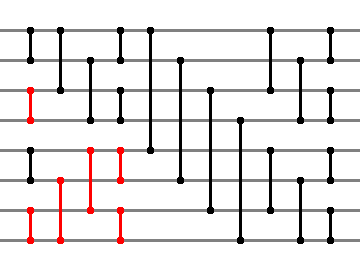
\includegraphics[width= \textwidth]{network.png}
			\end{block}
		\end{column}
	\end{columns}
\end{frame}

\begin{frame}{Randomized Data-Oblivious Sorting}
	\begin{itemize}
		\item Tilfældigt valgte sammenligninger
		\item Generelle algoritmer, dybde er ikke så vigtigt
		\item Nye algoritmer
			\begin{itemize}
				\item Randomized Shellsort (10)
				\item Annealing Sort (14)
			\end{itemize}
		\item Shaker Sort (87)
		\item Bedre køretider, ikke garanteret success
		\item Praktiske problemer
	\end{itemize}
\end{frame}


\begin{frame}<beamer:0>[noframenumbering]{Other Data-Oblivious Algorithms}
	\begin{itemize}
		\item Graf-algoritmer
		\begin{itemize}
			\item[] \mycite{ObliviousGraph}
		\end{itemize}
		\item Geometriske algoritmer
		\begin{itemize}
			\item[] \mycite{GraphGeoOblivious}
		\end{itemize}
		\item Mængde-Operationer
		\begin{itemize}
			\item[] \mycite{ObliviousSet}
		\end{itemize}
		\item En del flere \dots
	\end{itemize}
\end{frame}


\section{Algoritmer}

\subsection{Randomized Shellsort}

\begin{frame}{Randomized Shellsort}
	{\center \mycite{RandShellSort}}
	\begin{itemize}
		\item Køretid: $\Theta(n \log n)$
		\item Fejlrate: $O(n^{-\alpha})$
		\item Region Comparison
		\item $c$ og oprydning
	\end{itemize}
\end{frame}

\begin{frame}<beamer:0>[noframenumbering]{Region Comparison}
	\begin{block}{Region Comparison}
		\begin{algorithmic}
			\Procedure{RegionCompare}{$A, i, j, size$}
				\For{$1 \dots c$}
				\Comment $c$ is a predetermined constant
					\State $matching \gets \mathtt{shuffle}([0 \dots size-1])$
					\For{$k = 0 \dots size-1$}
						\State $\mathtt{Compare\mbox{-}Exchange}(A, i + k, j + matching[k])$
					\EndFor
				\EndFor
			\EndProcedure
		\end{algorithmic}
	\end{block}
\end{frame}

\begin{frame}<beamer:0>[noframenumbering]{Randomized Shellsort}
	\begin{block}{Randomized Shellsort}
 	\tiny
		\begin{algorithmic}
			\Procedure{RandomizedShellsort}{$A, n$}
				\For{$jump = n/2, n/4, n/8 \dots 1$}
					\For{$i = 0 \dots n/jump-2$}
					\Comment Shaker pass part 1
						\State $\mathtt{RegionCompare}(A, i\cdot jump, (i+1)\cdot jump, jump)$
					\EndFor
					\For{$i = n/jump-1 \dots 1$}
					\Comment Shaker pass part 2
						\State $\mathtt{RegionCompare}(A, (i-1)\cdot jump, i\cdot jump, jump)$
					\EndFor
					\For{$i = 0 \dots n/jump-4$}
					\Comment Brick pass part 1
						\State $\mathtt{RegionCompare}(A, i\cdot jump, (i+3)\cdot jump, jump)$
					\EndFor
					\For{$i = 0 \dots n/jump-3$}
					\Comment Brick pass part 2
						\State $\mathtt{RegionCompare}(A, i\cdot jump, (i+2)\cdot jump, jump)$
					\EndFor
					\For{$i = 0, 2, 4 \dots n/jump-2$}
					\Comment Brick pass part 3
						\State $\mathtt{RegionCompare}(A, i\cdot jump, (i+1)\cdot jump, jump)$
					\EndFor
					\For{$i = 1, 3, 5 \dots n/jump-3$}
					\Comment Brick pass part 4
						\State $\mathtt{RegionCompare}(A, i \cdot jump, (i+1)\cdot jump, jump)$
					\EndFor
				\EndFor
				\State $\mathtt{Clean-Up(A)}$
			\EndProcedure
		\end{algorithmic}
	\end{block}
\end{frame}

\subsection{Annealing Sort}

\begin{frame}{Annealing Sort}
	{\center \mycite{AnnealingSort}}
	\begin{itemize}
		\item Køretid: $\Theta(n \log n)$
		\item Fejlrate: $O(n^{-\alpha})$
		\item Annealing Sequence
			\begin{enumerate}
			\tiny
				\item $[(n/2, c), (n/2, c), (n/4, c), (n/4, c) \dots (q \log^6 n, c), (q \log^6 n, c)]$  ---- $q \geq 1$ og $c > 1$
				\item $[(q \log^6 n, r),((q/2) \log^6 n, r), ((q/4) \log^6 n, r) \dots (g \log n, r)]$ --- $q$ fra fase 1, $g \geq 1$,  og $r$ er $\Theta(\frac{\log n}{\log \log n})$
				\item $[(1,1), (1,1) \dots (1,1)]$ --- længde $g \log n$
		\end{enumerate}
		\item Mange konstanter
	\end{itemize}
\end{frame}

\begin{frame}<beamer:0>[noframenumbering]{Annealing Sort}
	\begin{block}{Annealing Sort}
		\scriptsize
		\begin{algorithmic}
			\Procedure{AnnealingSort}{$A, n$}
				\For {$(t, r)$ in Annealing Sequence}
					\For {$i = 0 \dots n-2$}
						\For{$j = 1 \dots r$}
							\State {$\mathtt{Compare\mbox{-}Exchange}(A, i, \mathtt{random\mbox{-}choice}([i+1: \min(i+t, n-1)]))$}
						\EndFor
					\EndFor
					\For {$i = n-1 \dots 1$}
						\For{$j = 1 \dots r$}
							\State {$\mathtt{Compare\mbox{-}Exchange}(A, \mathtt{random\mbox{-}choice}([\max(i-t, 0): i-1]), i)$}
						\EndFor
					\EndFor
				\EndFor
			\EndProcedure
		\end{algorithmic}
	\end{block}
\end{frame}

\subsection{Bitonic Sort}

\begin{frame}{Bitonic Sort}
	{\center \mycite{SNApplications}}
	\begin{itemize}
	\item Klassisk Sorteringsnetværk
	\item Bitoniske Sekvenser
	\item Køretid: $\Theta(n \log^2 n)$
	\item Dybde: $\Theta(\log^2 n)$
	\end{itemize}
\end{frame}

\begin{frame}<beamer:0>[noframenumbering]{Bitonic Merge}
	\begin{block}{Bitonic Merge}
		\begin{algorithmic}
			\Procedure{BitonicMerge}{$A, n$}
				\If {$n>1$}
					\For {$i = 0 \dots n/2-1$}
						\State {$\mathtt{Compare\mbox{-}Exchange}(A, i, i+n/2)$}
					\EndFor
					\State{$\mathtt{BitonicMerge}(A[0 \dots n/2-1], n/2)$}
					\State{$\mathtt{BitonicMerge}(A[n/2 \dots n-1], n/2)$}
				\EndIf
			\EndProcedure
		\end{algorithmic}
	\end{block}
\end{frame}

\begin{frame}<beamer:0>[noframenumbering]{Bitonic Sort}
	\begin{block}{Bitonic Sort}
			\begin{algorithmic}
				\Procedure{BitonicSort}{$A, n$}
					\If {$n>1$}
						\State{$\mathtt{BitonicSort}(A[0 \dots n/2-1], n/2)$}
						\State{$\mathtt{BitonicSort}(A[n/2 \dots n-1], n/2)$}
						\State{$\mathtt{Reverse}(A[0 \dots n/2-1])$}
						\State{$\mathtt{BitonicMerge}(A, n)$}
					\EndIf
				\EndProcedure
		\end{algorithmic}
	\end{block}
\end{frame}


\subsection{Odd-Even Mergesort}

\begin{frame}{Odd-Even Mergesort}
	{\center \mycite{SNApplications}}
	\begin{itemize}
	\item Klassisk Sorteringsnetværk
	\item Merging $A$ and $B$
		\begin{itemize}
			\item
				$C = {a_0,(b_0, b_1), (b_2, a_1), (a_2, b_3) \dots}$
			\item
				$C = {b_0, (b_1, a_0), (b_2, a_1), (b_3, b_4) \dots}$
		\end{itemize}
	\item Køretid: $\Theta(n \log^2 n)$
	\item Dybde: $\Theta(\log^2 n)$
	\end{itemize}
\end{frame}

\begin{frame}<beamer:0>[noframenumbering]{Odd-Even Merge}
	\begin{block}{Odd-Even Merge}
		\begin{algorithmic}
		\scriptsize
			\Procedure{OddEvenMerge}{$A, B, n$}
				\If {$n=1$}
					\State $C \gets [{A[0], B[0]}]$
					\State $\mathtt{Compare-Exchange}(C, 0, 1)$
				\Else
					\State {$odd \gets \mathtt{OddEvenMerge}(\mathtt{odd}(A),\mathtt{odd}(B), n/2)$}
					\State {$even \gets \mathtt{OddEvenMerge}(\mathtt{even}(A),\mathtt{even}(B), n/2)$}
					\For {$i = 0 \dots n/2-1} $
						\State {$C[2i] \gets even[i]$}
						\State {$C[2i+1] \gets odd[i]$}
					\EndFor
					\For {$i = 0 \dots n/2-2} $
						\State {$\mathtt{Compare\mbox{-}Exchange}(C, 2i+1, 2i+2)$}
					\EndFor
				\EndIf
			\EndProcedure
		\end{algorithmic}
	\end{block}
\end{frame}

\begin{frame}<beamer:0>[noframenumbering]{Odd-Even Mergesort}
	\begin{block}{Odd-Even Mergesort}
		\begin{algorithmic}
\Procedure{OddEvenMergeSort}{$A, n$}
\If {$n>1$}
	\State{$\mathtt{OddEvenMergeSort}(A[0 \dots n/2-1], n/2)$}
	\State{$\mathtt{OddEvenMergeSort}(A[n/2 \dots n-1], n/2)$}
	\State{$\mathtt{OddEvenMerge}(A[0 \dots n/2-1], A[n/2 \dots n-1], n)$}
\EndIf
\EndProcedure
\end{algorithmic}
	\end{block}
\end{frame}


\subsection{Shellsort Varianter}

\begin{frame}
	{\center \mycite{Shellsort}}
	\begin{itemize}
		\item Shellsort
			\begin{itemize}
				\item Mulig, men ikke egnet
				\item Mere et framework
			\end{itemize}
		\item Pratt's Shellsort
			\begin{itemize}
				\item $2^i3^j < n$ sekvens
				\item Ét enkelt løb per indgang i sekvensen, $\Theta(n \log^2 n)$
			\end{itemize}
		\item Shaker Sort
			\begin{itemize}
				\item $\floor{1.7^j}+1 < n$ sekvens
				\item Enkelt løb, op og ned, $\Theta(n \log n)$
				\item Ukendt fejlrate
			\end{itemize}
	\end{itemize}
\end{frame}

\begin{frame}<beamer:0>[noframenumbering]{Pratts Shellsort}
	{\center \mycite{PrattThesis}}
	\begin{block}{Pratts Shellsort}
		\begin{algorithmic}
		\small
			\Procedure{PrattSort}{$A, n$}
				\For {$i = n/2, n/4, n/8 \dots 1$}
					\State{$j \gets i$}
					\Do
						\For {$k = 0 \dots n-j-1$}
							\State {$\mathtt{Compare-Exchange}(A,k,k+j)$}
						\EndFor
						\State {$ j \gets 3j/2$}
					\doWhile {$j \% 3 == 0\ \text{and}\ j < n$}
				\EndFor
			\EndProcedure
		\end{algorithmic}
	\end{block}
\end{frame}

\begin{frame}<beamer:0>[noframenumbering]{Shaker Sort}
	{\center \mycite{Shakersort}}
	\begin{block}{Shaker Sort}
		\begin{algorithmic}
		\footnotesize
			\Procedure{ShakerSort}{$A, n$}
				\State {$\mathtt{Shuffle}(A)$} 
				\Comment{Shuffle is optional, but advised for general inputs.}
				\State {$seq \gets \mathtt{ShakerSequence}(n)$}
				\ForAll {$s\ \mathbf{in}\ seq$}
					\For {$i = 0 \dots n-s-1$}
						\State {$\mathtt{Compare-Exchange}(A,i, i+s)$}
					\EndFor
					\For {$i = n-1 \dots s$}
						\State {$\mathtt{Compare-Exchange}(A,i-s, i)$}
					\EndFor
				\EndFor
			\EndProcedure
		\end{algorithmic}
	\end{block}
\end{frame}


%
\section{Implementation and Optimization}

\begin{frame}{Praktiske Problemer}
	\begin{itemize}
		\item Randomized Shellsort og Annealing Sort
			\begin{itemize}
				\item PRNG
				\item Konstanter
			\end{itemize}
		\item Bitonic Sort og Odd-Even Mergesort
			\begin{itemize}
				\item Templates
				\item Odd-Even buffering
				\item Rekursivt layout
				\item Dobbelt-lag
			\end{itemize}
		\item Pratts Shellsort og Shaker Sort
			\begin{itemize}
				\item Inline sekvenser mod precomputing
			\end{itemize}
	\end{itemize}
\end{frame}

\begin{frame}{SIMD}
	\begin{itemize}
		\item SSE4.1 - 128 bit, 4x32 bit
			\begin{itemize}
				\item Registre
				\item \texttt{PMINSD / PMAXSD}
			\end{itemize}
		\item Data Alignment
			\begin{itemize}
				\item 16-byte aligned
				\item 16-byte unaligned
				\item Individuelle loads
			\end{itemize}
		\item Brugbart? Ja
	\end{itemize}
\end{frame}

\begin{frame}{CUDA}
	\begin{itemize}
		\item \textbf{C}ompute \textbf{U}nified \textbf{D}evice \textbf{A}rchitecture
		\item Data-Obliviousness
	\end{itemize}
	\begin{block}{Individuel Tilpasning}
		\begin{description}
			\item[Randomized Shellsort] CPU -> Texture Shuffle
			\item[Bitonic Sort] Wire Mapping, Shared memory
			\item[Odd-Even Mergesort] Speciel Remapping
			\item[Shellsort Varianter] 1 tråd per sub-sekvens
		\end{description}
	\end{block}
\end{frame}

\begin{frame}{OpenMP}
	\begin{itemize}
		\item OpenMP Basics
		\item \texttt{\#pragma omp \dots}
		\item Stort overhead
	\end{itemize}
	\begin{block}{Individuel Tilpasning}
		\begin{description}
			\item[Randomized Shellsort] 1 tråd shuffler, mange sammenligner
			\item[Bitonic Sort] Tasks
			\item[Odd-Even Mergesort] Tasks
			\item[Shellsort Varianter] Manuel scheduling grundet cache
		\end{description}
	\end{block}
\end{frame}


\section{Zig-Zag Sort}

\begin{frame}<beamer:0>[noframenumbering]{AKS}
	\mycite{AKS}
	\begin{itemize}
		\item Deterministisk $O(n \log n)$ netværk, $O(\log n) dybde$
		\item Upraktisk beskrivelse
		\item Horrible konstanter
		\item $\epsilon$-halvers
			\begin{itemize}
				\item $\epsilon k$ af de $k$ største elementer i første halvdel
				\item $O(n)$, stærkt afhængig af $\epsilon$
				\item Svær at implementere deterministisk
				\item Randomizeret udgave er simpel
			\end{itemize}
		\item Mange varianter
	\end{itemize}
\end{frame}

\begin{frame}{Zig-Zag Sort}
	\mycite{ZigZag}
	\begin{itemize}
		\item Deterministisk $O(n \log n)$ netværk, $\Theta(n \log n) dybde$
		\item Præcist beskrevet
		\item Meget bedre konstanter end AKS, men meget dybt
		\item Afhængig af $\epsilon$-halvers, men bedre $\epsilon$
	\end{itemize}
\end{frame}

\begin{frame}<beamer:0>[noframenumbering]{Zig-Zag Sort}
	\begin{block}{Zig-Zag Sort}
 	\tiny
 		\begin{algorithmic}
			\Procedure{ZigZagSort}{$A, n$}
				\State $ranges \gets [[0 \dots n-1]]$
				\For{$1 \dots \log n$}
					\State $new\_ranges \gets []$
					\For{$r$ in $ranges$}
						\State $left, right \gets \mathtt{split}(r)$
						\State $\mathtt{Reduce}(left, right)$
						\State $new\_ranges \gets new\_ranges \cup [left, right]$
					\EndFor
					\For{$i \gets 0 \dots |new\_ranges|-2$}
					 	\State $\mathtt{swap}(new\_ranges[i], new\_ranges[i+1])$
					 	\State $\mathtt{Reduce}(new\_ranges[i], new\_ranges[i+1])$
					\EndFor\For{$i \gets |new\_ranges|-1 \dots 1$}
					 	\State $\mathtt{swap}(new\_ranges[i-1], new\_ranges[i])$
					 	\State $\mathtt{Reduce}(new\_ranges[i-1], new\_ranges[i])$
					\EndFor
					\State $ranges \gets new\_ranges$
				\EndFor
			\EndProcedure
		\end{algorithmic}
	\end{block}
\end{frame}

\begin{frame}<beamer:0>[noframenumbering]{Zig-Zag Sort}
	\begin{block}{Reduce}
 		\begin{algorithmic}
			\Procedure{Reduce}{$A, B$}
				\If {$|A| + |B| \leq 8$}
					\State $Sorter(A \cup B)$
				\EndIf
				\State $\epsilon \mbox{-}\mathtt{Halver}(A,B)$
				\State $\mathtt{Attenuate}(A,B)$
			\EndProcedure
		\end{algorithmic}
	\end{block}
\end{frame}

\begin{frame}<beamer:0>[noframenumbering]{Zig-Zag Sort}
	\begin{block}{Attenuate}
 		\begin{algorithmic}
 		\footnotesize
			\Procedure{Attenuate}{$A, B$}
				\If {$|A| + |B| \leq 8$}
					\State $Sorter(A \cup B)$
				\EndIf
				\State $(A_1, A_2), (B_1, B_2) \gets \mathtt{split}(A), \mathtt{split}(B)$
				\State $\epsilon \mbox{-}\mathtt{Halver}(A_1,A_2)$
				\State $\epsilon \mbox{-}\mathtt{Halver}(B_1,B_2)$
				\State $\epsilon \mbox{-}\mathtt{Halver}(A_2,B_1)$
				\State $\mathtt{Attenuate}(A_2,B_1)$
				\State $(A^*_1, A^*_2), (B^*_1, B^*_2) \gets \mathtt{split}(A_2), \mathtt{split}(B_1)$
				\State $\epsilon \mbox{-}\mathtt{Halver}(A^*_1,A^*_2)$
				\State $\epsilon \mbox{-}\mathtt{Halver}(B^*_1,B^*_2)$
				\State $\epsilon \mbox{-}\mathtt{Halver}(A^*_2,B^*_1)$
				\State $\mathtt{Attenuate}(A_2,B_1)$
			\EndProcedure
		\end{algorithmic}
	\end{block}
\end{frame}

\begin{frame}{Zig-Zag Sort}
	\begin{itemize}
		\item Faktiske tal: $\approx 50 cn \log n$, hvis $\epsilon$-halver er $cn$
		\item Praktisk implementation, $n = 1024$, \#sammenligninger:
			\begin{itemize}
				\item Zig-Zag Sort - $7056780$
				\item Odd-Even Mergesort - $24063$
			\end{itemize}
	\end{itemize}
\end{frame}


\section{Eksperimenter}

\begin{frame}{Nye Algoritmer}
	\begin{columns}[T]
		\begin{column}{.55\textwidth}
			Sammenligninger
			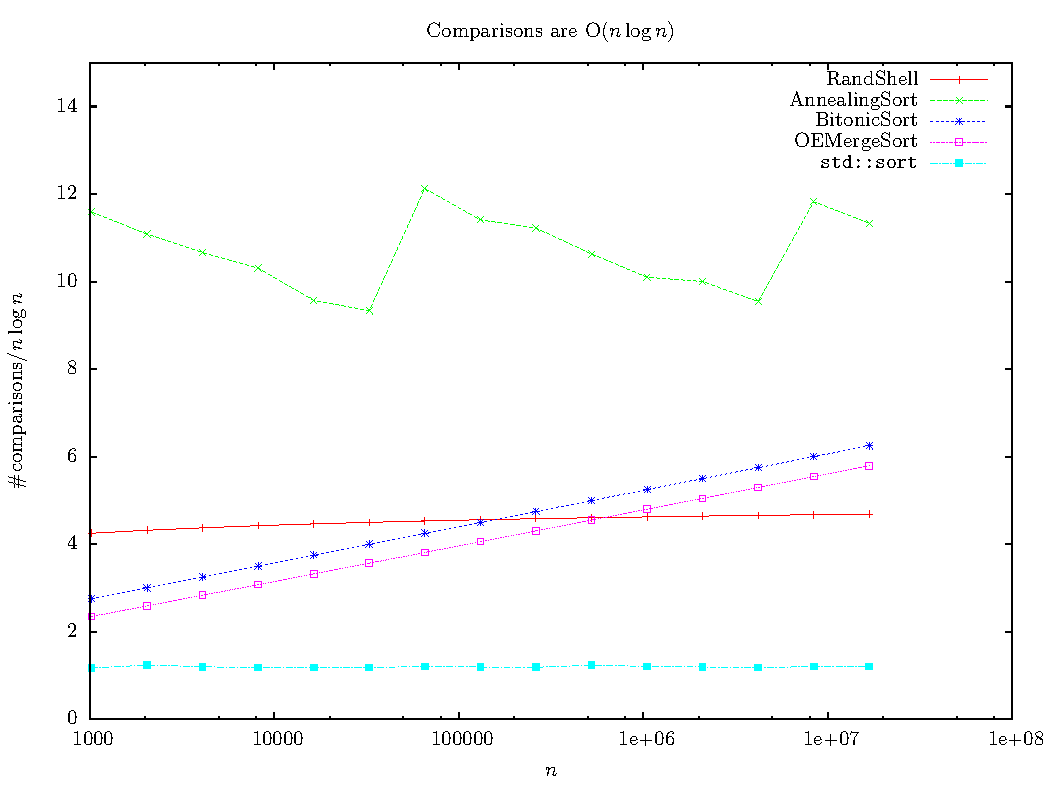
\includegraphics[width= \textwidth]{graphs/Performance/nlogncomparisons.pdf}
		\end{column}
		\begin{column}{.55\textwidth}
			Tid
			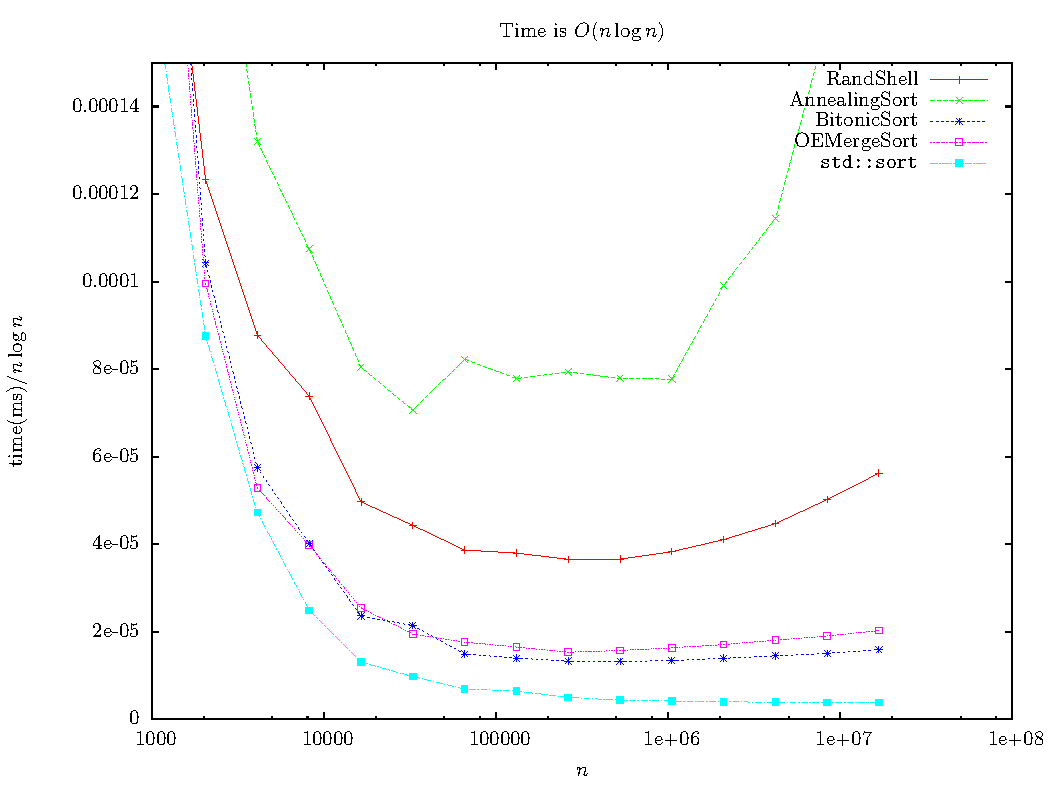
\includegraphics[width= \textwidth]{graphs/Performance/nlogntime.pdf}
		\end{column}
	\end{columns}
\end{frame}

\begin{frame}{Nye Algoritmer}
	\begin{columns}[T]
		\begin{column}{.55\textwidth}
			Instruktioner
			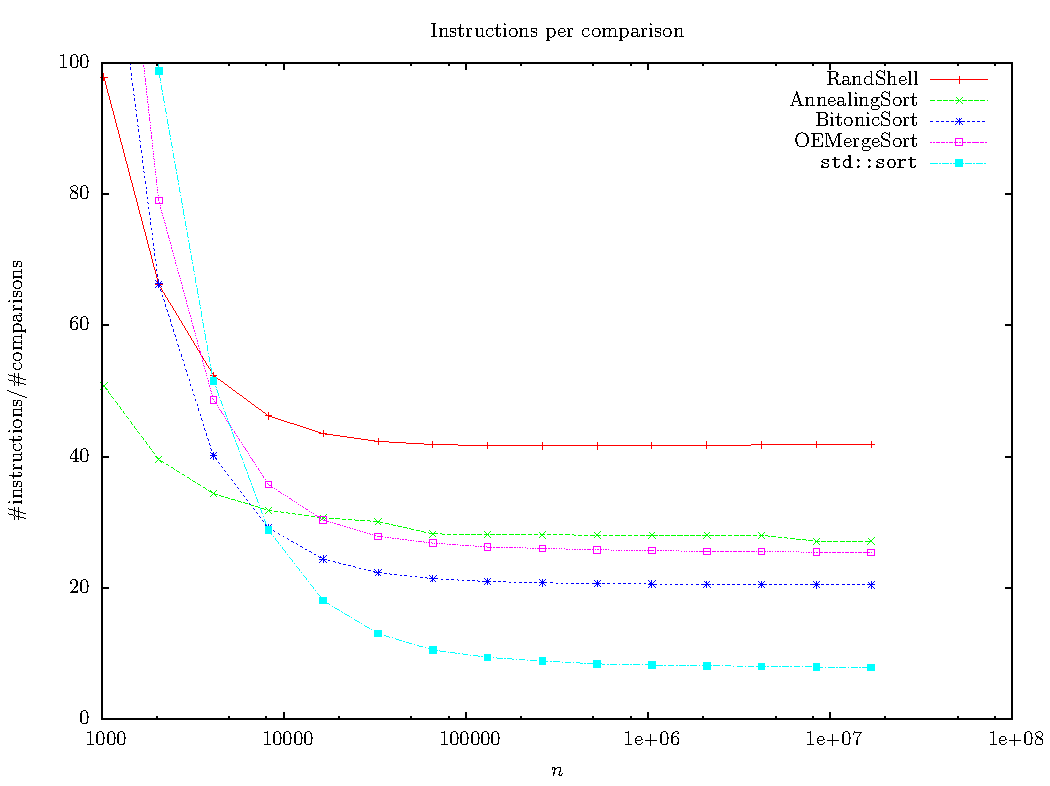
\includegraphics[width= \textwidth]{graphs/Performance/instructionscomparison.pdf}
		\end{column}
		\begin{column}{.55\textwidth}
			Cache-Misses
			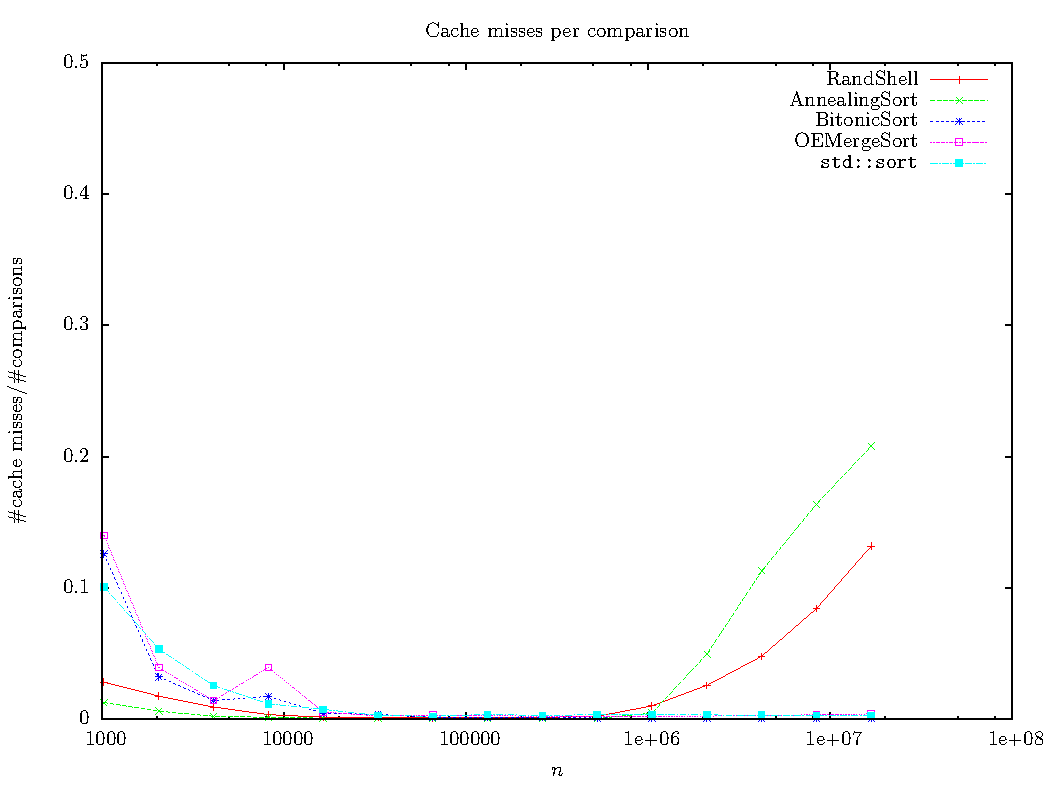
\includegraphics[width= \textwidth]{graphs/Performance/cache-misses.pdf}
		\end{column}
	\end{columns}
\end{frame}

\begin{frame}{Shellsorts}
	\begin{columns}[T]
		\begin{column}{.48\textwidth}
			Sammenligninger
			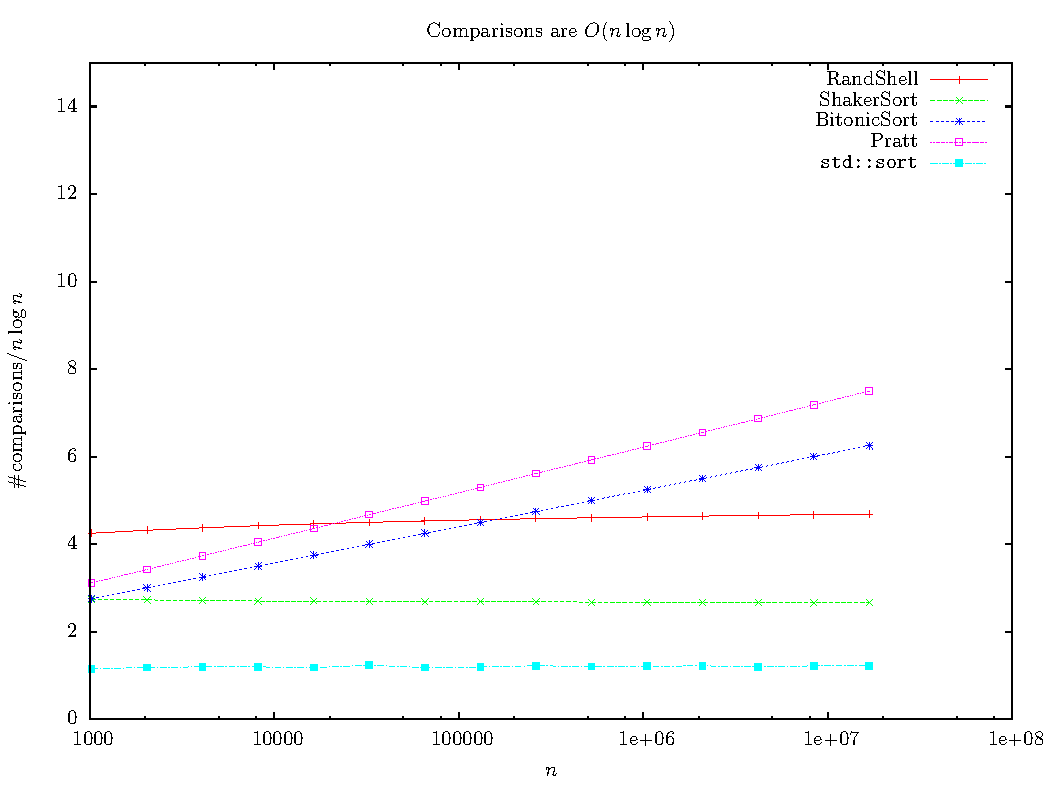
\includegraphics[width= \textwidth]{graphs/Shellsorts/nlogncomparisons.pdf}
		\end{column}
		\begin{column}{.55\textwidth}
			Tid
			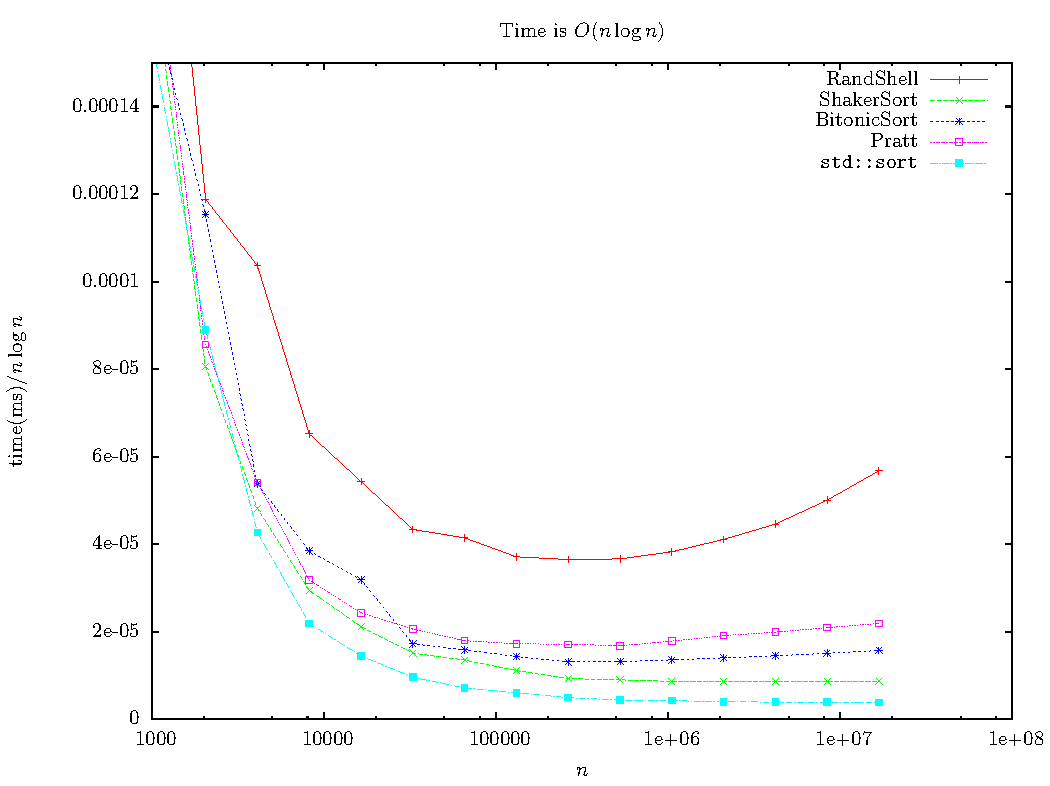
\includegraphics[width= \textwidth]{graphs/Shellsorts/nlogntime.pdf}
		\end{column}
	\end{columns}
\end{frame}

\begin{frame}{Shellsorts}
	\begin{columns}[T]
		\begin{column}{.55\textwidth}
			Instruktioner
			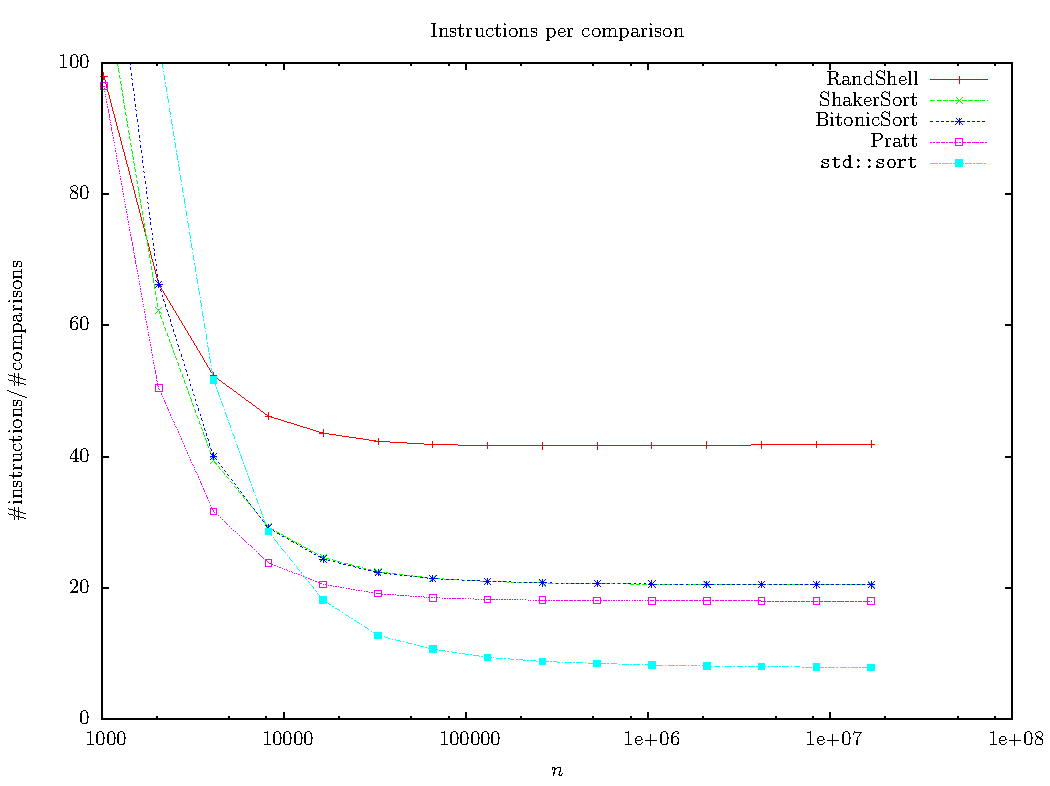
\includegraphics[width= \textwidth]{graphs/Shellsorts/instructionscomparison.pdf}
		\end{column}
		\begin{column}{.55\textwidth}
			Cache-Misses
			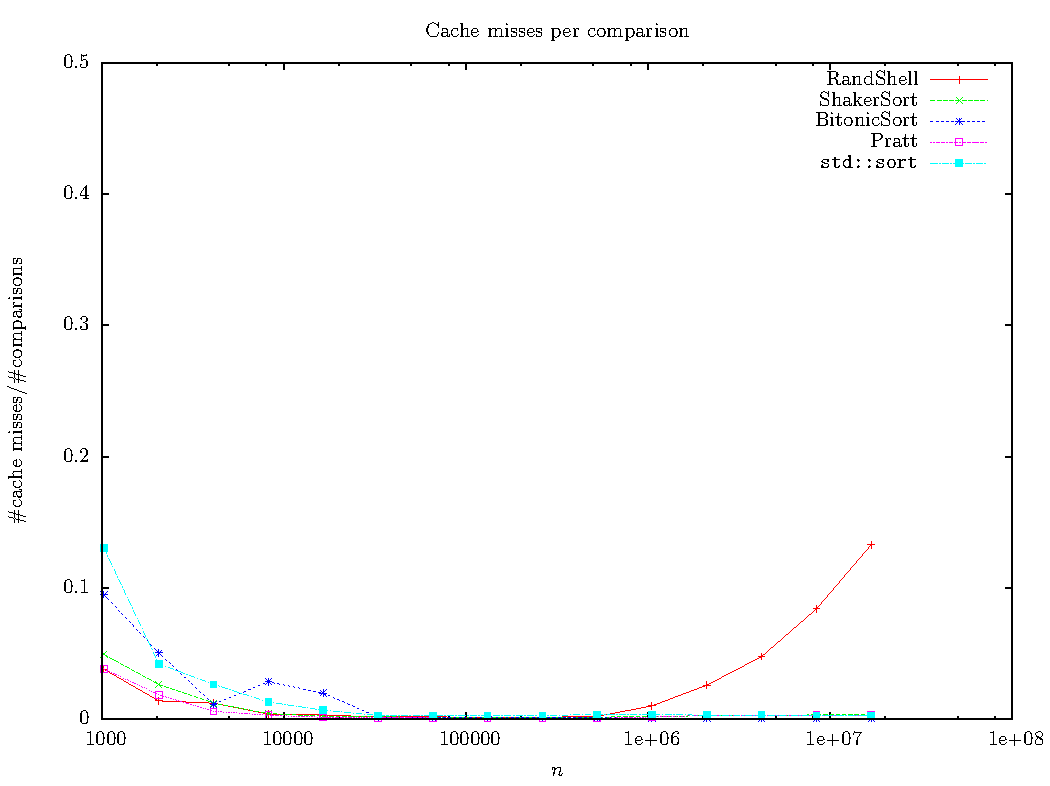
\includegraphics[width= \textwidth]{graphs/Shellsorts/cache-misses.pdf}
		\end{column}
	\end{columns}
\end{frame}

\begin{frame}{SIMD}
	\begin{itemize}
		\item SSE4.1 - 128 bit, 4x32 bit
			\begin{itemize}
				\item Registre
				\item \texttt{PMINSD / PMAXSD}
			\end{itemize}
		\item Data Alignment
			\begin{itemize}
				\item 16-byte aligned
				\item 16-byte unaligned
				\item Individuelle loads
			\end{itemize}
		\item Brugbart? Ja
	\end{itemize}
\end{frame}

\begin{frame}{SIMD}
	\begin{columns}[T]
		\begin{column}{.55\textwidth}
			Instruktioner
			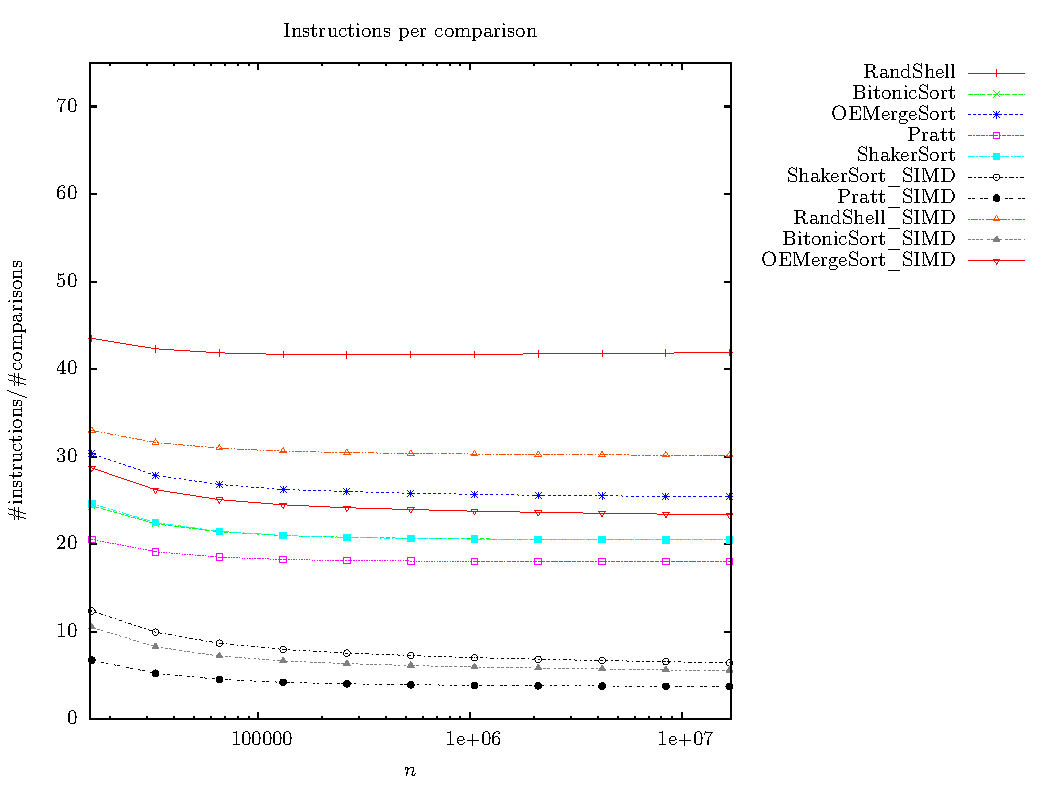
\includegraphics[width= \textwidth]{graphs/SIMD/instructionscomparison.pdf}
		\end{column}
		\begin{column}{.55\textwidth}
			Tidsændring
			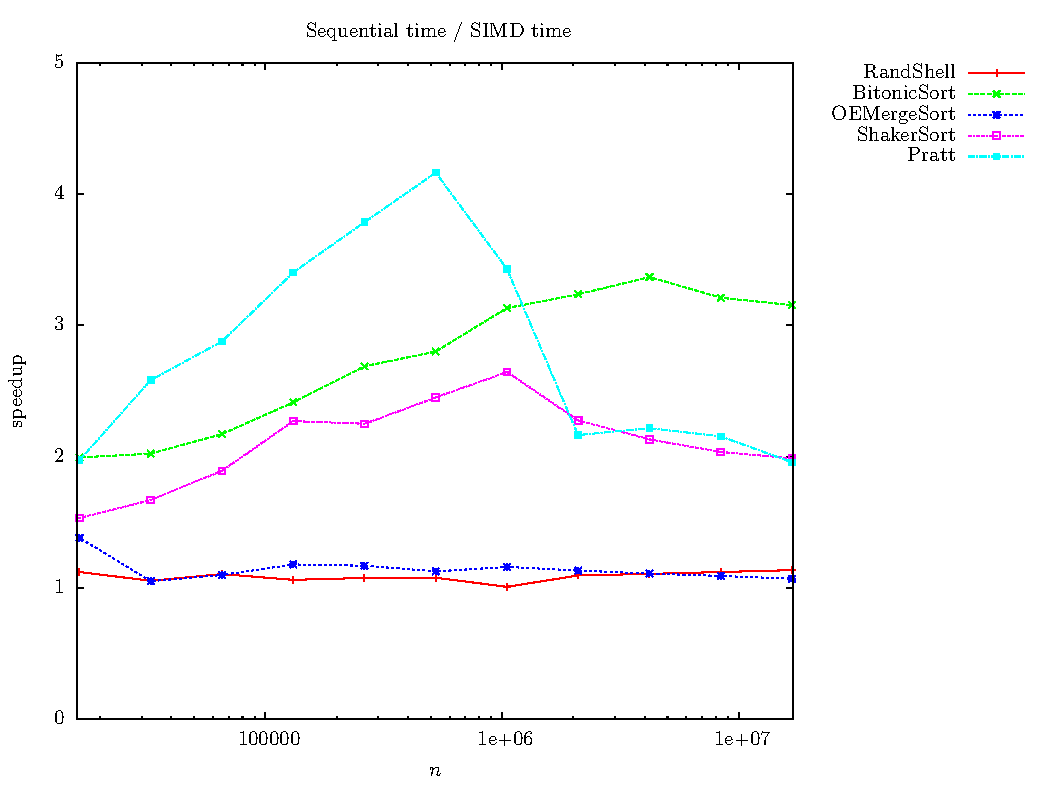
\includegraphics[width= \textwidth]{graphs/SIMD/timediff.pdf}
		\end{column}
	\end{columns}
\end{frame}

\begin{frame}{CUDA}
	\begin{itemize}
		\item \textbf{C}ompute \textbf{U}nified \textbf{D}evice \textbf{A}rchitecture
		\item Data-Obliviousness
	\end{itemize}
	\begin{block}{Individuel Tilpasning}
		\begin{description}
			\item[Randomized Shellsort] CPU -> Texture Shuffle
			\item[Bitonic Sort] Wire Mapping, Shared memory
			\item[Odd-Even Mergesort] Speciel Remapping
			\item[Shellsort Varianter] 1 tråd per sub-sekvens
		\end{description}
	\end{block}
\end{frame}


\begin{frame}{CUDA - Quadro FX 880M
}
	\begin{columns}[T]
		\begin{column}{.55\textwidth}
			Tid
			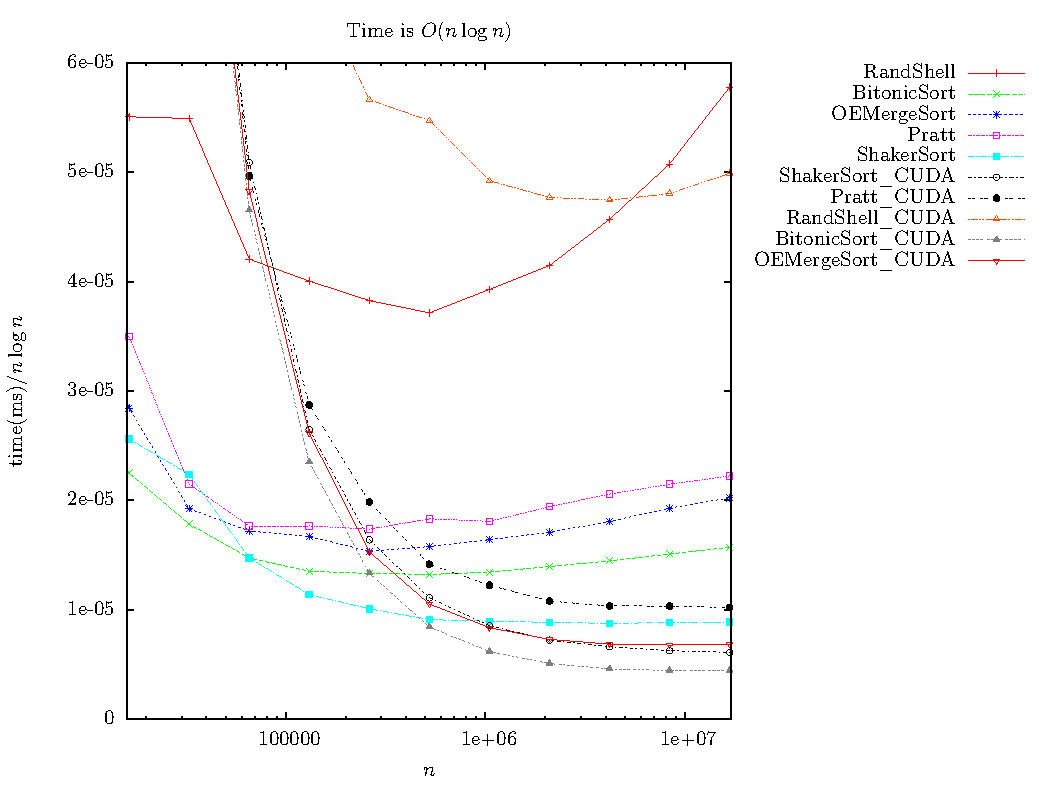
\includegraphics[width= \textwidth]{graphs/CUDA/nlogntime.pdf}
		\end{column}
		\begin{column}{.55\textwidth}
			Tidsændring
			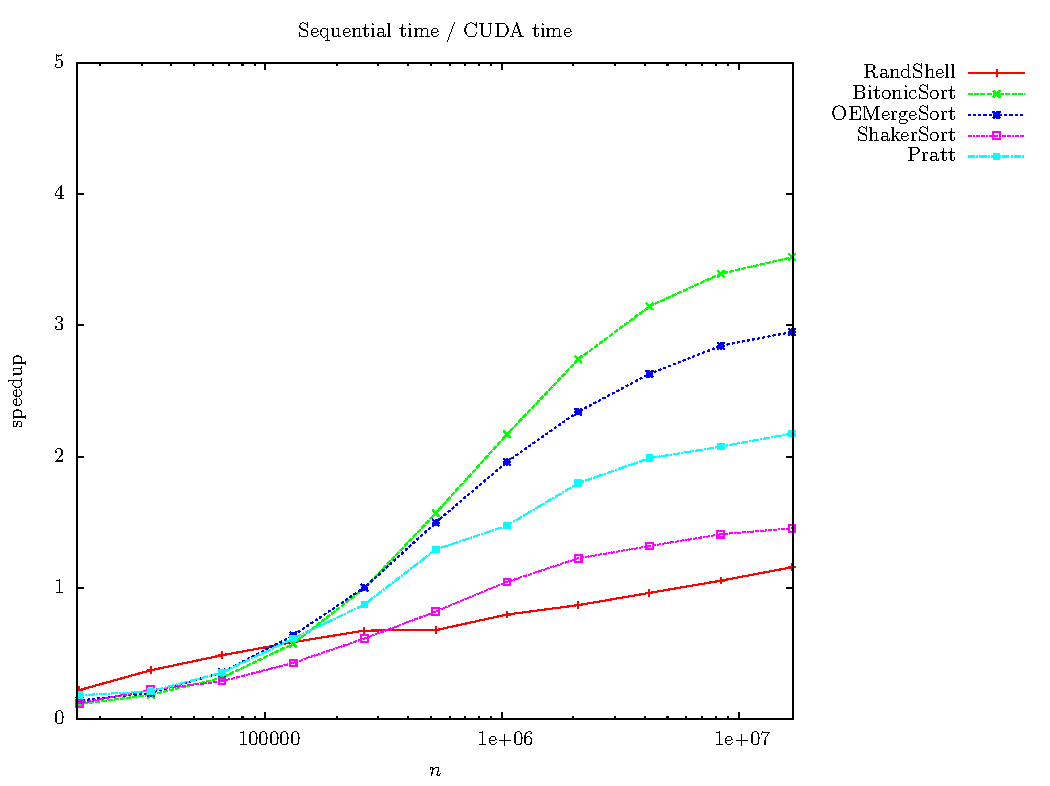
\includegraphics[width= \textwidth]{graphs/CUDA/timediff.pdf}
		\end{column}
	\end{columns}
\end{frame}


\begin{frame}{CUDA - GTX 880M}
	\begin{columns}[T]
		\begin{column}{.55\textwidth}
			Tid
			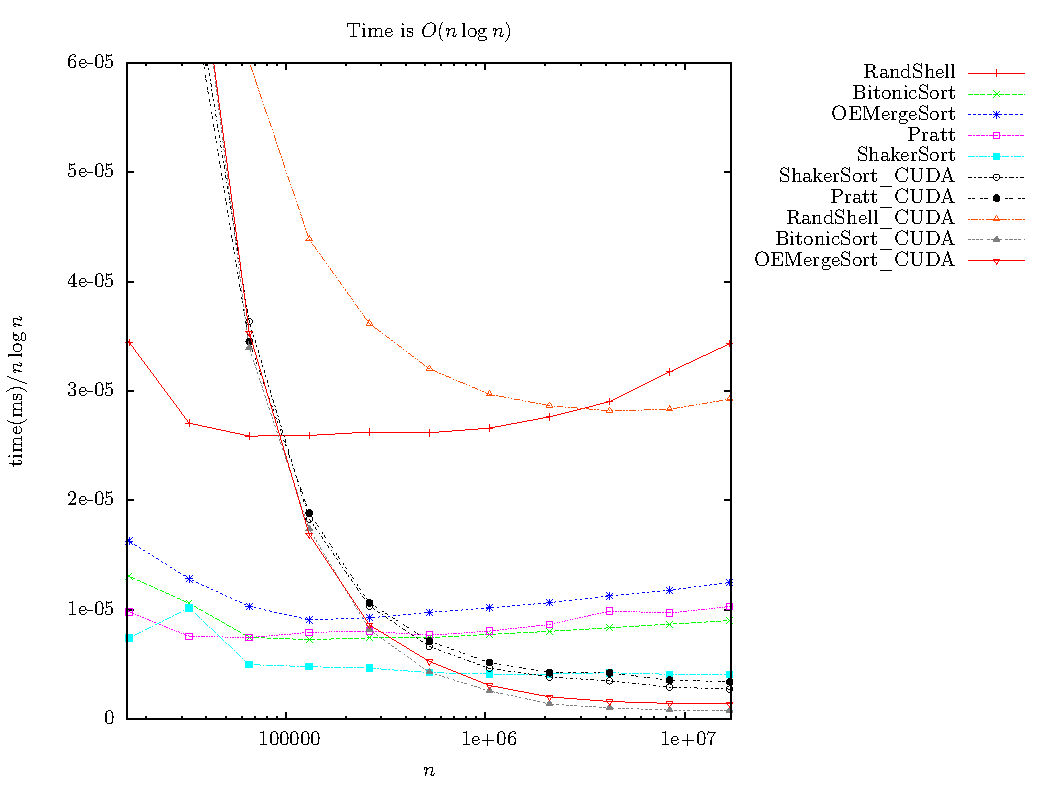
\includegraphics[width= \textwidth]{graphs/CUDAHueg/nlogntime.pdf}
		\end{column}
		\begin{column}{.55\textwidth}
			Tidsændring
			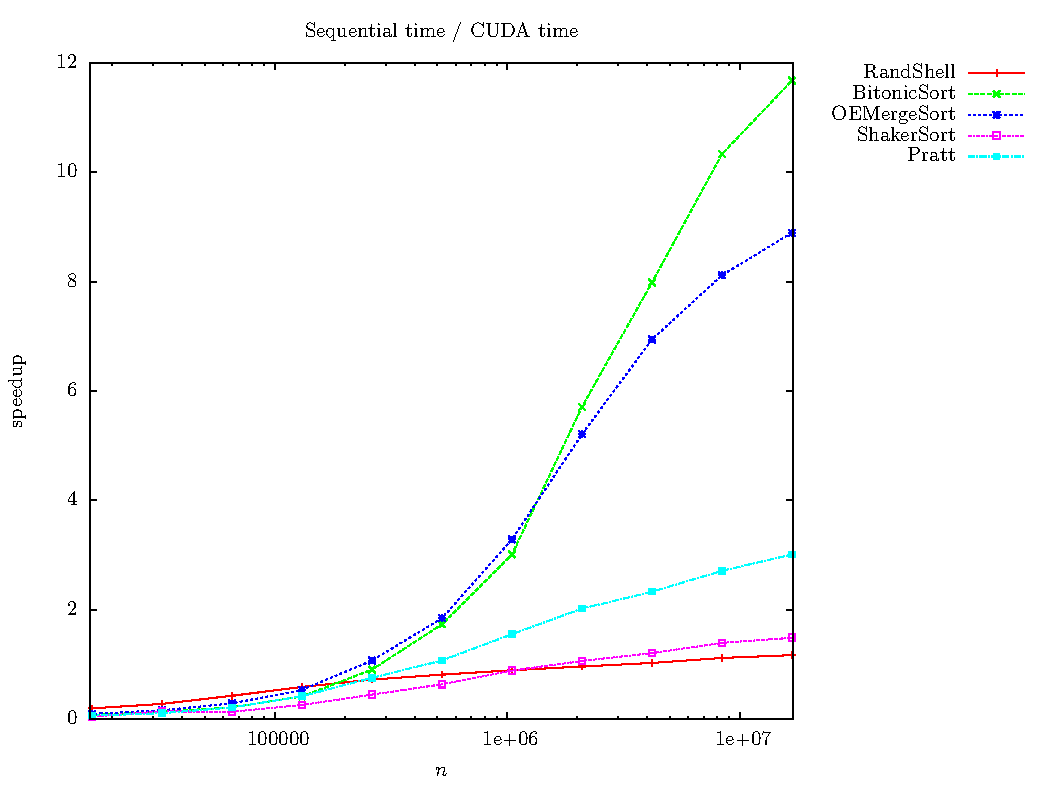
\includegraphics[width= \textwidth]{graphs/CUDAHueg/timediff.pdf}
		\end{column}
	\end{columns}
\end{frame}


\begin{frame}{OpenMP}
	\begin{itemize}
		\item OpenMP Basics
		\item \texttt{\#pragma omp \dots}
		\item Stort overhead
	\end{itemize}
	\begin{block}{Individuel Tilpasning}
		\begin{description}
			\item[Randomized Shellsort] 1 tråd shuffler, mange sammenligner
			\item[Bitonic Sort] Tasks
			\item[Odd-Even Mergesort] Tasks
			\item[Shellsort Varianter] Manuel scheduling grundet cache
		\end{description}
	\end{block}
\end{frame}


\begin{frame}{OpenMP}
	\begin{columns}[T]
		\begin{column}{.55\textwidth}
			Tidsændring
			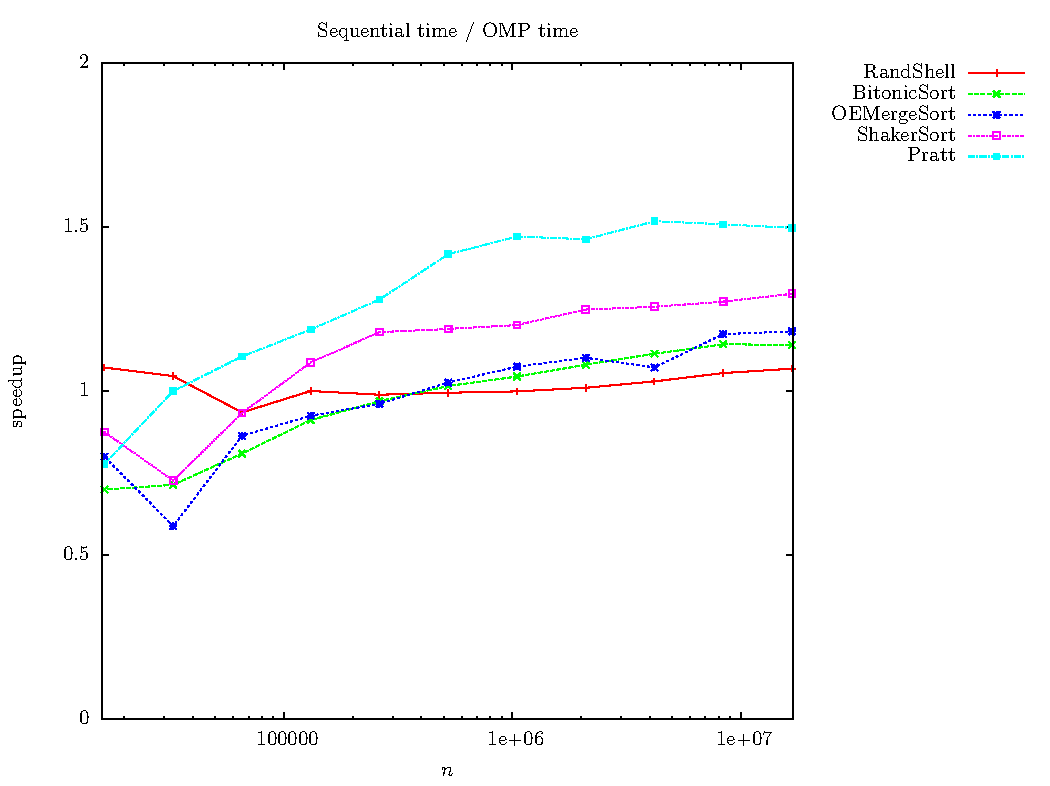
\includegraphics[width= \textwidth]{graphs/OMP/timediff.pdf}
		\end{column}
		\begin{column}{.55\textwidth}
			Instruktionsændring
			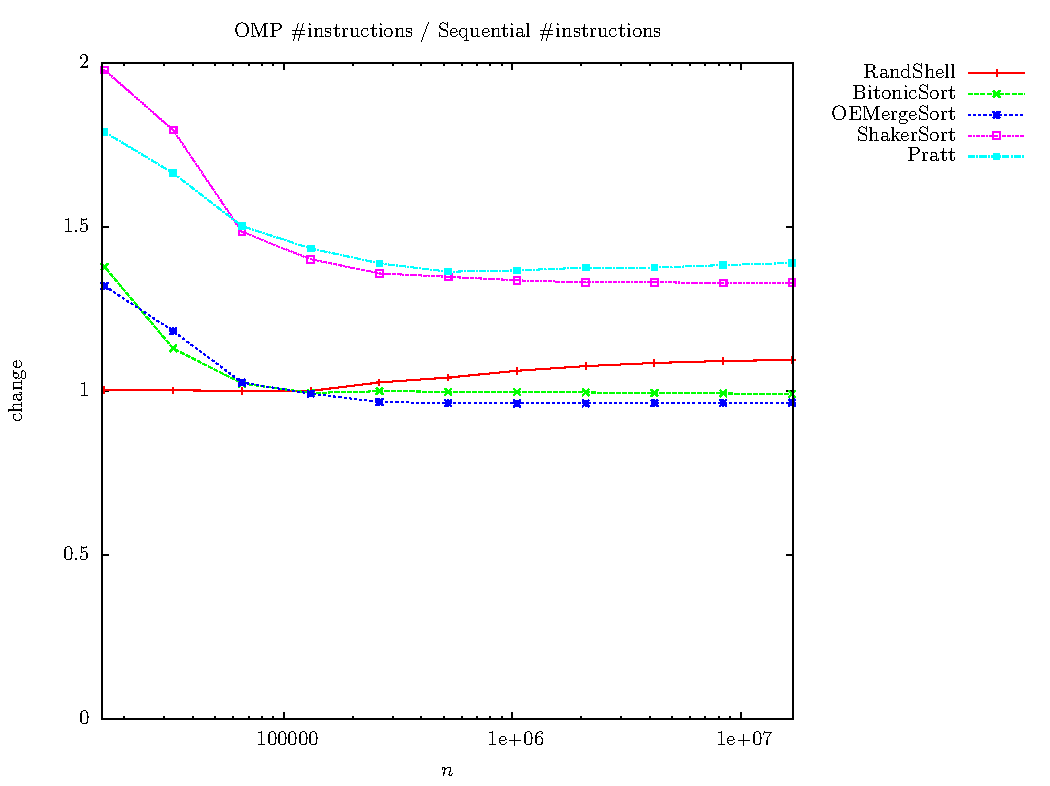
\includegraphics[width= \textwidth]{graphs/OMP/instrdiff.pdf}
		\end{column}
	\end{columns}
\end{frame}

\begin{frame}{OpenMP}
	\begin{columns}[T]
		\begin{column}{.55\textwidth}
			Cacheændring
			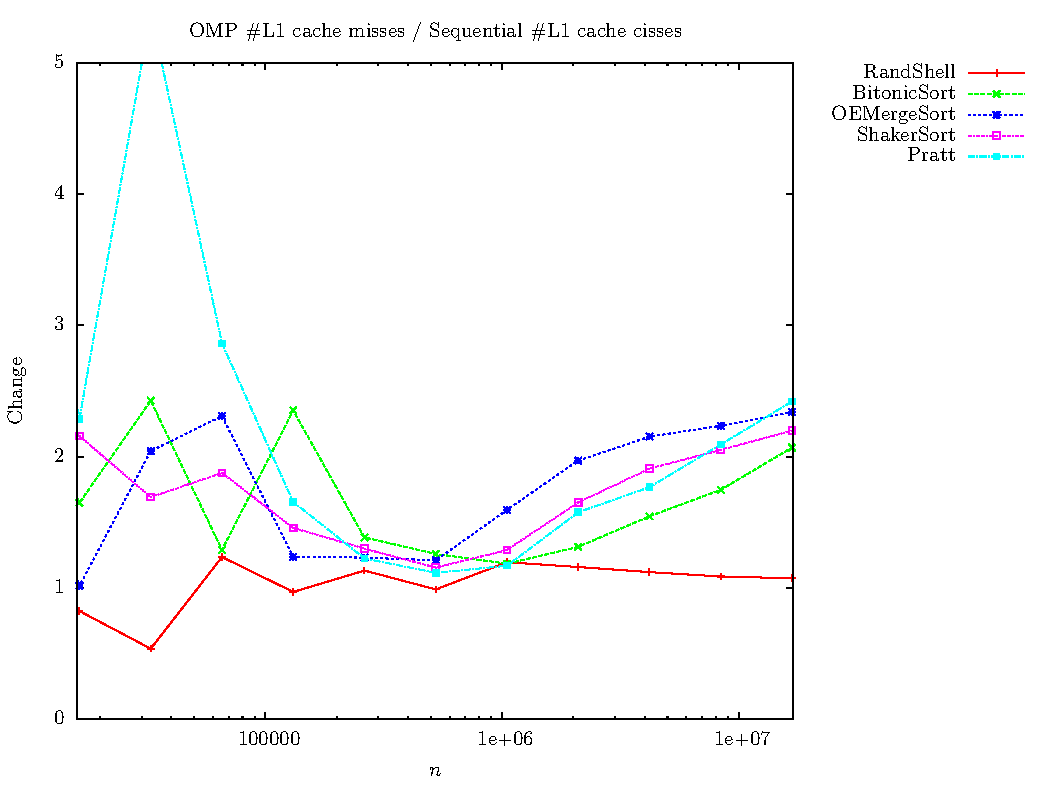
\includegraphics[width= \textwidth]{graphs/OMP/cachediff.pdf}
		\end{column}
		\begin{column}{.55\textwidth}
			Branchændring
			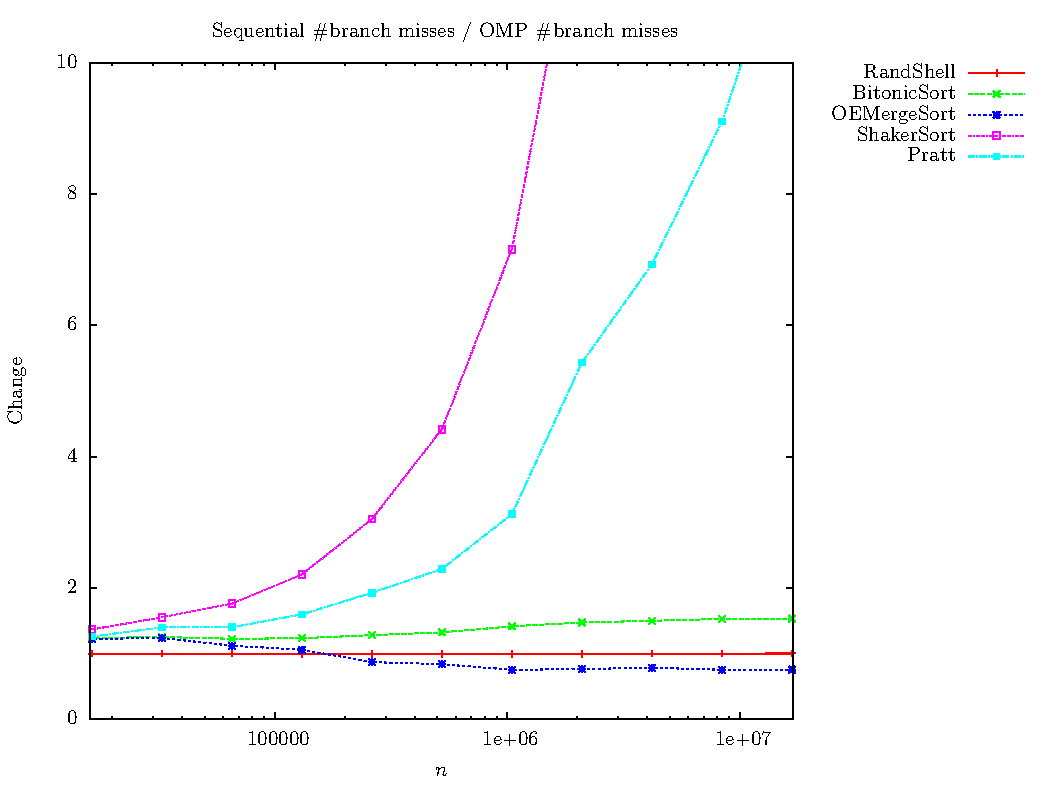
\includegraphics[width= \textwidth]{graphs/OMP/branchdiff.pdf}
		\end{column}
	\end{columns}
\end{frame}


\section{Konklusioner}

\begin{frame}
			\begin{itemize}
				\item De nye algoritmer er smarte, men fungerer dårligt i praksis
				\item Ikke meget at gøre ved det
				\item Men! Nye teknikker gør de gamle algorithmer hurtige
			\end{itemize}
			\begin{tabular}{|l|c c c c|}
\showrowcolors
\hline
& Base & SIMD & CUDA & OpenMP  \\ \hline
Randomized Shellsort & 22.6 & 20.2 & \textbf{20.1} & 21.5\\ 
Bitonic Sort & 6.41 & 2.02 & \textbf{1.80} & 5.61\\ 
Odd-Even Mergesort & 8.15 & 7.60 & \textbf{2.76} & 7.02\\ 
Pratt's Shellsort & 8.82  & 4.50 & \textbf{4.11} & 5.85 \\ 
Shaker Sort & 3.48 & \textbf{1.75} & 2.46 & 2.65\\ 
Annealing Sort & \textbf{67.3} & - & - & - \\ \hline
\end{tabular}
\end{frame}

%\section{Automatic Vectorization}

\begin{frame}{Automatic Vectorization}
	\begin{itemize}
		\item SIMD, på compile-time
		\item Kæmpe arbejde at pille med en compiler
		\item Simulering, log sammenligninger: \texttt{CE(0,8), CE(1,9) \dots}
		\item Alignment
			\begin{itemize}
				\item Aligned
				\item Unaligned
				\item Individuelle loads
			\end{itemize}
		\item Varierende vide af registre
	\end{itemize}
\end{frame}

\begin{frame}[fragile]{Shaker Sort Vectorized}
	\begin{columns}
		\begin{column}{0.48\textwidth}
			\begin{block}{basis}
			\tiny
				\begin{verbatim}
0: CE(0,25)
1: CE(1,26)
2: CE(2,27)
3: CE(3,28)
4: CE(4,29)
5: CE(5,30)
6: CE(6,31)
7: CE(6,31)
8: CE(5,30)
9: CE(4,29)
10: CE(3,28)
11: CE(2,27)
12: CE(1,26)
13: CE(0,25)
14: CE(0,15)
15: CE(1,16)
16: CE(2,17)
17: CE(3,18)
18: CE(4,19)
19: CE(5,20)
20: CE(6,21)
21: CE(7,22)
...
				\end{verbatim}
			\end{block}		
		\end{column}
		\begin{column}{0.48\textwidth}
			\begin{block}{vectorized}
			\tiny
				\begin{verbatim}
0: CE4U(0, 25)
1: CE(4, 29)
2: CE(5, 30)
3: CE(6, 31)
4: CE4U(3, 28)
5: CE(2, 27)
6: CE(1, 26)
7: CE(0, 25)
8: CE4U(0, 15)
9: CE4U(4, 19)
...
				\end{verbatim}
				\vspace{2.5cm}
			\end{block}
		\end{column}
	\end{columns}
\end{frame}

\begin{frame}{Resultater}
	\begin{itemize}
		\item Klar reduktion i operationer for mange algoritmer
	\end{itemize}
	\scriptsize
	\begin{tabular}{|l c c c c|}
\showrowcolors
\hline
Algorithm & Scalar & Aligned & Unaligned & Shuffled \\
\hline
Randomized Shellsort & 215048 & 213758 & 213617 & 72182\\

Recursive Odd-Even MergeSort & 139263 & 139263 & 139263 & 57954\\

Layered Odd-Even Mergesort & 139263 & 67074 & 67074 & 34818\\

Recursive Bitonic Sort & 159744 & 75264 & 75264 & 56835\\

Layered Bitonic Sort & 159744 & 75264 & 75264 & 39936\\

Pratt's Shellsort & 183634 & 87889 & 55138 & 55114\\

Shaker Sort & 125348 & 121730 & 55934 & 55934\\

Annealing Sort & 524160 & 524160 & 524160 & 524160\\
\hline
\end{tabular}
\end{frame}

\begin{frame}{Layering}
	\begin{itemize}
		\item Rækkefølgen af sammenligner er kun relevant indefor samme index
		\item Læg sammenligniner så tidligt som muligt, reducer dybden af netværket.
	\end{itemize}
	\small
	\begin{algorithmic}
		\Procedure{LayerOrdering}{$ops, n$}
			\State {$Depths \gets [-1, -1,...,-1] \text{ of lenght } n$}
			\State {$Ordering \gets []$}
			\For {$(i, j)\ \mathbf{in}\ ops$}	
				\State{$depth \gets \max(Depths[i], Depths[j])+1$}
				\State{$Depths[i], Depths[j] \gets depth, depth$}
				\State{$Ordering\ {+}{=}\ [(depth, i, j)]$}
			\EndFor
			\State{$\mathtt{Sort}(Ordering)$}
			\State{$\mathbf{return} [(i,j)\ \mathbf{for}\ (depth, i, j)\ \mathbf{in}\ Ordering]$}
		\EndProcedure
	\end{algorithmic}
\end{frame}

\begin{frame}{Layering Resultater}
	\begin{itemize}
		\item Klar ændring
	\end{itemize}
	\scriptsize
	\begin{tabular}{|l c c c c|}
\hline
Algorithm & Sequential & Aligned & Unaligned & Shuffled \\
\hline
Randomized Shellsort & 215048 & 213773 & 213560 & 64520\\

Recursive Odd-Even Mergesort & 139263 & 71676 & 70143 & 34818\\

Layered OddEven Mergesort & 139263 & 67074 & 67074 & 34818\\

Recursive Bitonic Sort & 159744 & 75264 & 75264 & 39936\\

Layered Bitonic Sort & 159744 & 75264 & 75264 & 39936\\

Pratt' Shellsort & 183634 & 92467 & 55312 & 48217\\

Shaker Sort & 125348 & 121730 & 71222 & 55916\\

Annealing Sort & 524160 & 524160 & 524154 & 197529\\
\hline
\end{tabular}
\end{frame}

\end{document}
